\section{Writing Modular Code}
\label{sec:modular_code}

\subsection{Analog Input}
\label{sub:analog_input}
\begin{frame}[fragile]
	\frametitle{Analog Input}
	AnalogIn operates almost identically to DigitalIn:
	\begin{lstlisting}[numbers=none]
		AnalogIn in(PinName pin);
	\end{lstlisting}
	\vfill
	You can access the value by treating it like a variable or with a function:
	\begin{lstlisting}[]
		float value = in;
		float value = in.read();
		unsigned short value = in.read_u16();
	\end{lstlisting}
	1 and 2 are identical and return a float in the range [0.0 -- 1.0].\\
	3 returns an unsigned short in the range [0x0000 -- 0xFFFF].
\end{frame}

\begin{frame}
	\frametitle{Using Potentiometers}
	\begin{columns}[T]
		\begin{column}{0.5\textwidth}
			A potentiometer functions as an adjustable voltage divider:
			\begin{itemize}
				\item One leg connects to 3.3v
				\item One leg connects to Gnd
				\item Wiper connects to an analog pin
			\end{itemize}
			The wiper varies between 0 and 3.3v as you turn the knob.
		\end{column}
		\begin{column}{0.5\textwidth}
			%TODO potentiometer schematic
			%TODO hookup picture
		\end{column}
	\end{columns}
\end{frame}

\begin{frame}[fragile]
	\frametitle{Analog Input Demo}
	\begin{columns}[T]
		\begin{column}{0.5\textwidth}
			Create a new program:
			\begin{itemize}
				\item AnalogIn connected to potentiometer
				\item Serial port connected to USB
				\item Print the analog value to serial
				\item Try using format specifiers with printf
			\end{itemize}
		\end{column}
		\pause
		\begin{column}{0.5\textwidth}
			\lstinputlisting[title=Analog.cpp]{code/modular_code/analog.cpp}
		\end{column}
	\end{columns}
\end{frame}

\subsection{PWM Output}
\label{sub:pwm_output}
\begin{frame}
	\frametitle{PWM Output}
	\begin{columns}[c]
		\begin{column}{0.5\textwidth}
			Pulse Width Modulation encodes a signal by varying the width of a series of pulses.\\
			\bigskip
			Used for:
			\begin{itemize}
				\item Analog output (filtered)
				\item Servo position control
				\item Load control
			\end{itemize}
		\end{column}
		\begin{column}{0.5\textwidth}
			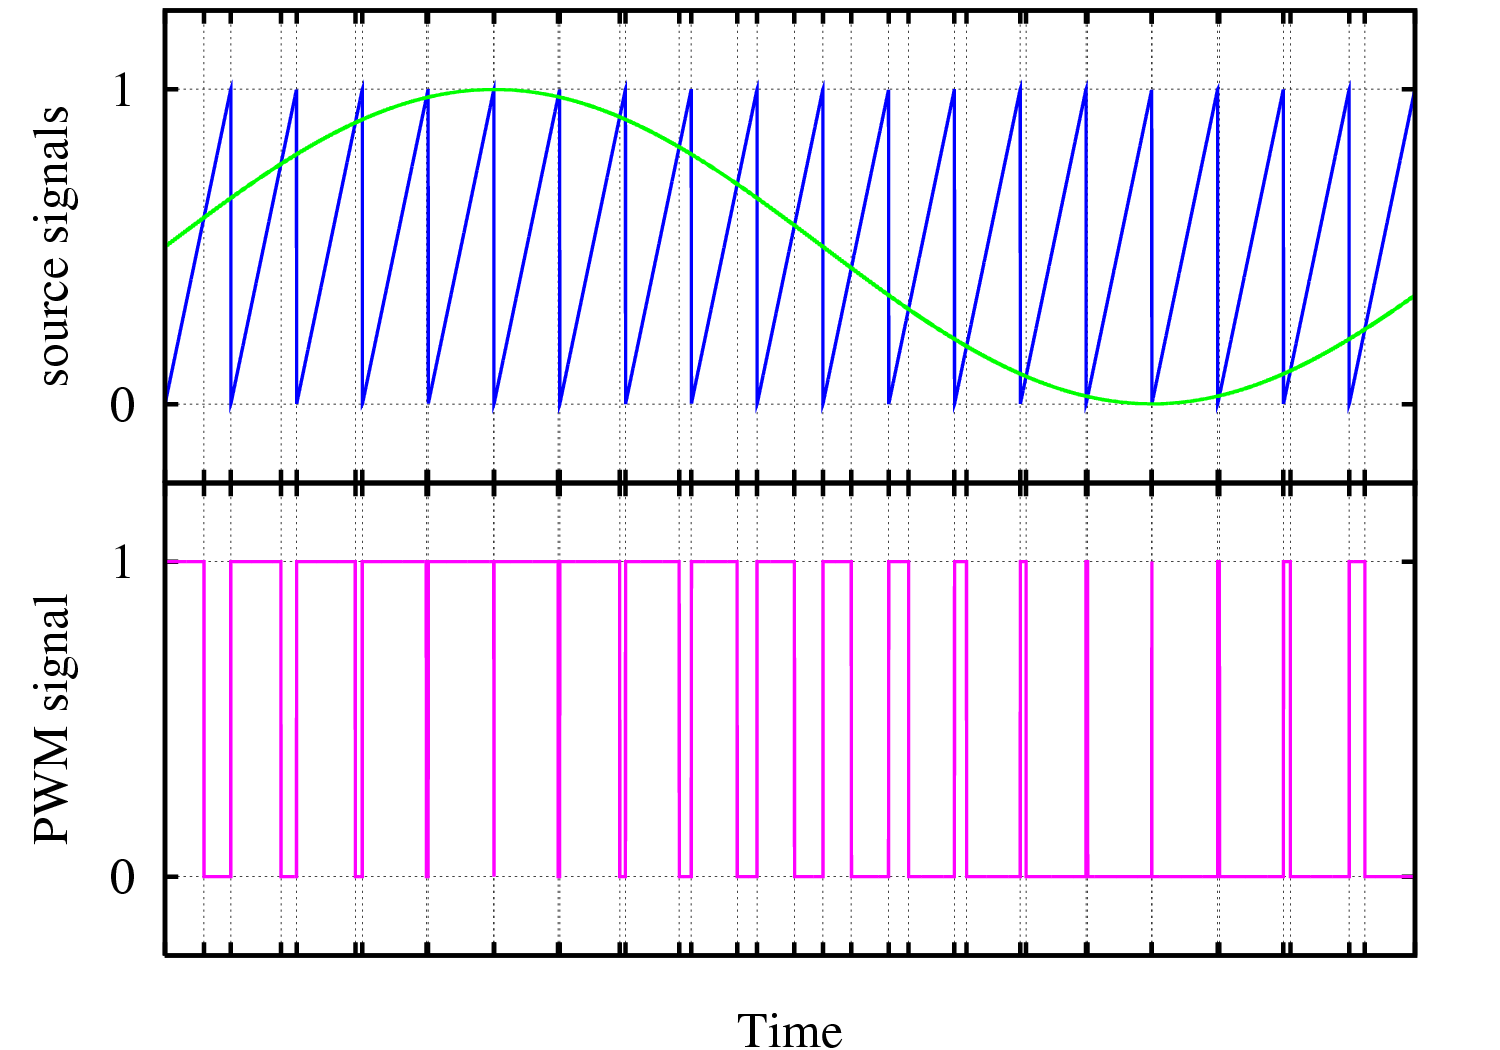
\includegraphics[width=\linewidth]{pwm}
		\end{column}
	\end{columns}
	\ccbysa{http://commons.wikimedia.org/wiki/File:Pwm.png}{CyrilB}
\end{frame}

\begin{frame}[fragile]
	\frametitle{PWM Output}
	You can use PwmOut on any purple pin marked PWM:
	\begin{lstlisting}[numbers=none]
		PwmOut out(PinName pin);
	\end{lstlisting}
	\vfill
	\begin{columns}[T]
		\begin{column}{0.5\textwidth}
			The period is controlled with:
			\begin{lstlisting}[numbers=none]
				out.period(float seconds);
				out.period_ms(int ms);
				out.period_us(int us);
			\end{lstlisting}
			and defaults to 0.02 seconds.
		\end{column}
		\begin{column}{0.5\textwidth}
			The pulse width is controlled with:
			\begin{lstlisting}[numbers=none]
				out = 0.5;
				out.write(float value);
				out.pulsewidth(float seconds);
				out.pulsewidth_ms(int ms);
				out.pulsewidth_us(int us);
			\end{lstlisting}
			The first two methods take a float in the range [0.0 -- 1.0].
		\end{column}
	\end{columns}
	\vfill
	Use whichever methods suit your application best.
\end{frame}

\begin{frame}[fragile]
	\frametitle{PWM Demo}
	\begin{columns}[T]
		\begin{column}{0.5\textwidth}
			Create a new program:
			\begin{itemize}
				\item PwmOut connected to the LED
				\item A loop changing the brightness of the LED
				\pause
				\item Brightness is proportional to duty cycle
				\item Don't forget to slow your program down!
				\pause
				\item Try playing with the period
			\end{itemize}
		\end{column}
		\begin{column}{0.5\textwidth}
			\lstinputlisting[title=Pwm.cpp]{code/modular_code/pwm.cpp}
		\end{column}
	\end{columns}
\end{frame}

\begin{frame}
	\frametitle{PWM Notes}
	Be aware that the same PWM signal may be exposed on several pins, you can only use one at a time.
	\vfill
	PWMx/y is the y-th channel of the x-th timer. All PWM's on a single timer must have the same frequency/period but can have different duty cycles.
	\vfill
	PWMx/yN has the same period and duty cycle as PWMx/y but is inverted.
\end{frame}

\subsection{Classes}
\label{sub:classes}
